\section{Discussion}
\label{sec:discussion}

\subsection{Heel- and toe-strike do not appear to produce different vertical ground reaction forces (GRF) or body accelerations}

One hypothesis I set out to test was that heel-strike would produce larger ground reaction forces (GRFs) or body accelerations. This was not supported by data from the force plate kymograph (\fref{fig:results:forceplate}) or from body center of mass accelerations during running (\fref{fig:results:accel}), which showed little difference between the vertical GRFs and $Y$ component accelerations. As a result, I conclude shin splints are not just caused by grossly higher forces in heel-strike running. In retrospect, it seems reasonable to expect this as the weight of the runner has not changed and the overall stride parameters (stride frequency, period, length, and duty cycle), while posessing some small changes, are not wildly different (\fref{fig:results:stride} and \fref{tab:results:stride}). 



\subsection{Toe-strike (forefoot strike) may produce larger horizontal GRFs on pushoff?}

The force plate kymograph data suggest that forefoot-strike produces a larger horizontal ground reaction force upon pushoff. The improvised instrumentation I used was too crude to observe the magnitude and timing of horizontal ground reaction forces; and an alternative explanation could be that the pavers used in the force plate have nonlinear friction in one direction that resulted in the observed patterns (yellow arrows in \fref{fig:results:forceplate}). However, given that for the same speed, toe-striking used a shorter duty cycle (\fref{fig:results:stride} and \fref{tab:results:stride}) it seems reasonable that, with less contact time with the ground per step, the horizontal ground reaction forces to keep moving forward at the same speed would need to be higher during some part of the cycle.



\subsection{Kinematic differences between heel- and toe-strike suggest a mechanism for higher loads in the lower leg}

Without a ``smoking gun'' in my force plate and accelerometer readings, I had to take a closer look at kinematic differences between the two running styles. The hip and knee joint angles look similar between the heel- and forefoot-strike (\fref{fig:results:jointangles}C-F), however, there are clear differences in the foot angles (\fref{fig:results:jointangles}A-B). In heel-strike, the leg impacts the ground with the heel, while the foot is dorsiflexed. During forefoot-strike, on the other hand, the leg impacts the ground first with the toe, and the foot remains plantar flexed for nearly all of stance.

When I look closely at the kinematic tracings of figures~\ref{fig:results:heelpretty} and \ref{fig:results:toepretty}, it appears that during heel-strike as the heel comes in contact with the ground, the lower leg (knee to ankle, containing tibia, fibula, etc) is closely aligned with the line of action of the ground reaction force to the hip (compare line from hip to triangles versus the alignment of the lower leg in \fref{fig:results:heelpretty}). In contrast, during forefoot-strike as the toe comes in contact with the ground, the lower leg is not aligned with the line of action of the ground reaction force to the hip (line from hip to triangle is not aligned with lower leg in \fref{fig:results:toepretty}). When I compared these angles (\fref{fig:results:contactangles}), the differences between the two treatments were significant. While the gross, overall forces and accelerations may not be different between the two styles, the fine details of forces as experienced by particular parts of the leg could be very different during key instances of the stride; in heel-strike the lower leg must take all of the load as a compressive shock load at the start of every stance phase, while in forefoot-strike the leg acts more compliant and is able to share the load not just on the lower leg, but also the foot, the upper leg, and the muscles and tendons crossing several joints (including the gastrocnemius and the achilles tendon). 

Data in other kinematic studies are consistent with my findings; \citet{viitasalo1983some} found runners with shin splints had greater angular displacements and experienced greater Achilles tendon angles during shin splints, as well as greater angular displacement between heel strike and the maximal everted position. \citet{mizrahi2000effect} found that kinematic changes in long distance runners during fatigue included lower stride frequency, joint angle differences, increased hip vertical excursion, and higher accelerations of the shank, which they interpreted as conssitent with higher impact accelerations and increasd risk of overload injuries. Adoption of a more compliant gait might be expected to reduce mechanical forces transmitted through the skeleton but incurs a higher metabolic cost \citep{mcmahon1987groucho}. \citet{giandolini2013impact} found a combination of compliant shoes, increased stride frequency, and shifting to a forefoot strike were effective in attenuating the foot-ground impact. They also found that forefoot strike was associated with pre-activation of the gastrocnemius lateralis, preparing it to act as a spring or shock absorber during contact. 


\subsection{Limitations of my study, and findings of other researchers}
Because of the global COVID-19 pandemic, I was limited to using an improvised force plate kymograph.  With better instrumentation, I would have been able to examine the horizontal and vertical ground reaction forces in more detail. Using such instrumentation, \citet{dickinson1985measurement} demonstrated a shock wave propagates through the skeletal system following heel strike and suggests it was not seen in previous measurements because of adequate shock absorption provided by running shoes, but became readily apparent in barefoot runners (\fref{fig:discussion}). The impact peak is also seen in seen in the data of \citep{chan1994foot, boyer2015rearfoot, lieberman2010foot}. \citet{knorz2017three} combined left and right force plate measurements and 3D kinematics to resolve the detailed ground reaction forces and to map them to stress patterns in the ankle, knee, and hip joint, concluding that forefoot and rearfoot strike were associated with different 3D stress patterns with no global advantage of one strike pattern over the other. Rearfoot strike had peak during initial contact as seen by others, but had a lower maximum peak force during stance. \citet{boyer2015rearfoot} concluded that not all lower extremity loading variables are lower with a forefoot strike or when running barefoot; switching to a forefoot strike may not alleviate certain pain or help runners avoid injury. \citet{boyer2015rearfoot} considers a more viable option may be to shorten one’s stride length 10\%.
\begin{figure}
\begin{center}
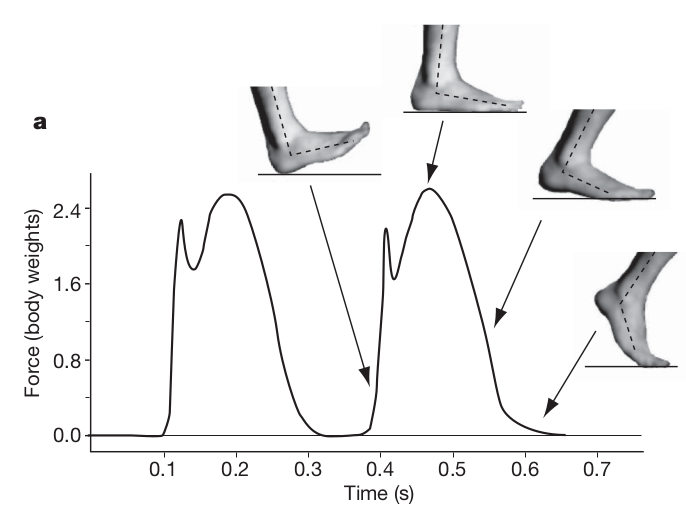
\includegraphics[width=3in]{figures/lieberman1.png}
\includegraphics[width=3in]{figures/lieberman2.png}
\end{center}
\caption{Spike present in ground reaction forces at contact for heel-strike (left); spike absent during forefoot-strike barefoot running (right), from \citep{lieberman2010foot}. With higher resolution force plate measurements, I would have been able to resolve the spike.}
\label{fig:discussion}
\end{figure}

\citet{lieberman2010foot} studied barefoot versus habitually shod runners with an eye towards evolution of locomotion in early homonids. They showed that habitually barefoot endurance runners often land on the fore-foot (fore-foot strike) before bringing down the heel, but they sometimes land with a flat foot (mid-foot strike) or, less often, on the heel (rear-foot strike) \citep{lieberman2010foot}. In contrast, habitually shod runners mostly rear-foot strike, facilitated by the elevated and cushioned heel of the modern running shoe \citep{lieberman2010foot}. \citet{lieberman2010foot} performed kinematic and kinetic analyses (similar to mine) that showed that even on hard surfaces, barefoot runners who fore-foot strike generate smaller collision forces than shod rear-foot strikers. As observed in my kinematics data, the differences result primarily from a more plantarflexed foot at landing and more ankle compliance during impact, which \citet{lieberman2010foot} attribute to decreasing the effective mass of the body that collides with the ground. Fore-foot- and mid-foot-strike gaits were probably more common when humans ran barefoot or in minimal shoes, and may protect the feet and lower limbs from some of the impact-related injuries now experienced by a high percentage of runners \citep{lieberman2010foot}.

Through simple biomechanical observations I was able to do at home while sheltering in place during COVID-19, I was able to observe forces, accelerations, and kinematic differences between two different running styles. Further study could continue to look at peaks in compressive forces during contact, as well as periodic function representation of joint angles for bipedal and polypedal locomotion. 